\documentclass[workingdraft,endnotes]{usetex-v1}
% 1. workingdraft:
%
%       For initial submission and shepherding.  Features prominent
%       date, notice of draft status, page numbers, and annotation
%       facilities.  The three supported annotation macros are:
%               \edannote{text}         -- anonymous annotation note
%               \begin{ednote}{who}     -- annotation note attributed
%                 text                          to ``who''
%               \end{ednote}
%               \HERE                   -- a marker that can be left
%                                               in the text and easily
%                                               searched for later
%
% In addition, the option "endnotes" permits the use of the
% otherwise-disabled, Usenix-deprecated footnote{} command in
% documents.  In this case, be sure to include a
% \makeendnotes command at the end of your document or
% the endnotes will not actually appear.
%
\usepackage{preamble}




\begin{document}

\title{mGTK}

\docstatus{Submitted to USENIX'04 (FREENIX track)}

\author{
\authname{Ken Friis Larsen}
%\authaddr{Your Department}
%\authaddr{Your Institution}
%\authaddr{ Your City, State, ZIP}
\authurl{\url{ken@friislarsen.net}}
%\authurl{\url{http://host.dom/yoururl}}
\and
\authname{Henning Niss}
\authaddr{Department of Innovation}
\authaddr{IT University of Copenhagen}
\authaddr{Denmark}
\authurl{\url{hniss@it.edu}}
\authurl{\url{http://www.it.edu/people/hniss}}
%
} % end author

\maketitle

\begin{abstract}
  We describe \mgtk a language binding that makes the graphical
  toolkit \gtk, written in C, accessible for programs written in the
  programming language Standard~ML (\sml).  This is not a trivial task
  because \gtk is based on an object-oriented and \sml is functional
  language with a non--object-oriented type system.  In this paper we
  describe how it is possible to encode a single-inheritance
  class-hierarchy using \sml's type system and we describe how we
  machine-generate most of the library to utilize the limited
  man-power of the project.
\end{abstract}



\section{Introduction}
\label{sec:intr-backgr}

This section gives a brief introduction to \sml and \gtk, and present
an overview of the rest of the paper.

\begin{ednote}{Ken}
  * Hvad med at motivere og forklare hvorfor vi vil have et grafisk lib
  til SML.

  * SML er ikke OO (tester Gtk+-folkenes "hypotese")
\end{ednote}

\subsection{Standard ML}

\begin{ednote}{Ken}
  Take one.  It is crap but is it here
\end{ednote}

Standard ML (\sml) is a functional language with imperative features
widely used for teaching and in research.  It is roughtly on the same
level of abstraction as Python or Scheme, but in contrast to Python
and Scheme, which are \emph{dynamically typed}, is \sml
\emph{statically typed} like Java and C++ which means that type errors
are detected at \emph{compile time} in contrast to \emph{run time}.
Despite \sml being statically typed, it is not necessary for the
programmaer to provide type annotations because \sml features
\emph{type inference} which means that the compiler reconstruct type
annotations as needed.  \sml also features algebraric datatypes,
pattern-matching, tuples and records, first-class and anonymous
functions, exception handling, immutable data types and updatable
references, abstract data types, and parametric modules, but it is
outside the scope of this paper to introduce all these features,
instead we refer the interested reading to one of the fine textbooks
\cite{Hansen-Rischel:1999,Paulson:1996}.

\begin{ednote}{Ken}
  Skulle vi have et lille fac og fib eksempel?
\end{ednote}

\sml is one of the few languages with a formal definition
\cite{Milner:1997:Definition}.  The definition defines \sml in 93
pages of mathematical notation and English prose.  The book is not
meant as tutorial for the language, its existence is rather to provide
an implementation-independent formulation of \sml.  This formal
definition means that it is possible to write substantial applications
in \sml which are not dependent on a specific compiler, also there
areseveral mature \sml implementations with widely different
implementation strategies ranging from byte-code interpreters with
interactive \emph{read--eval--print--loops} (REPLs) to aggresively
optimizing whole-program compilers targeting native code.



\subsection{\gtk}
\label{sec:gtk}


\begin{ednote}{Ken}
  * Gtk+ er interessant (og C var et godt
    impl. valg)  
\end{ednote}
  

\subsection{Overview of this paper}
\label{sec:overview-this-paper}



\section{Running Example}
\label{sec:example}

\begin{ednote}{Henning}
  I moved this section up a bit in order to introduce SML lingo
  early on.
\end{ednote}

\begin{ednote}{Henning}
  This ended up being to long, I think.
  It is easier to just write stuff down now, and then shorten
  afterwards.
\end{ednote}

Figure~\ref{fig:hello-world} shows a deliberately simple Hello World
example using \mgtk. It illustrates (1) how to get the toolkit
initialized using \texttt{GtkBasis.init} (from a module containing
basic \gtk functionality not related to specific widgets), (2) how to
construct new widgets (using module \texttt{Window} for the Window
widget, and \texttt{Button} for the Button widget), and (3) how to
connect signals to widgets (using module \texttt{Signal}).
\begin{figure*}[htbp]
\begin{centering}
\begin{verbatim}
fun hello _ = print "Hello World\n"

fun main _ =
    let val _ = 
           GtkBasis.init(CommandLine.name()::CommandLine.arguments())
        val window = Window.new ()
        val button = Button.new_with_label "Hello World"
    in  Signal.connect window (Widget.delete_event_sig (fn _ => false))
      ; Signal.connect window (Widget.destroy_sig GtkBasis.main_quit)
      ; Signal.connect button (Button.clicked_sig hello)
      ; Container.add window button
      ; Widget.show_all window
      ; GtkBasis.main() 
    end

val _ = main()
\end{verbatim}
\caption{Hello World in \mgtk.\label{fig:hello-world}}
\end{centering}
\end{figure*}

In the figure we use the following \sml constructs
(see a textbook on \sml for further examples;
\cite{Hansen-Rischel:1999,Paulson:1996} for example). The construct
\texttt{fun} \textit{foo} \textit{x} \texttt{=} \textit{exp} declares
a function \textit{foo} that has one formal parameter \textit{x} and
function body \textit{exp}; \texttt{fn} \textit{x} \texttt{=>}
\textit{exp} denotes a similar \emph{anonymous} function. If one does
not care about the parameter, one can use the \emph{wildcard}
\texttt{\_}. The construct \texttt{let}~\texttt{val} \textit{x} \texttt{=}
\textit{exp} declares the identifier \textit{x} to be bound to the
value obtained by evaluating \textit{exp}. If the only reason
for evaluating \textit{exp} is any potential side effect, one
can again use the wildcard \texttt{\_}. Expressions evaluated for
their side effects can also be sequentialized using \texttt{;}.
The value \texttt{()}, ``unit'', can be used as is and is also used
as the return value of purely side-effecting functions.
Finally, \textit{Foo}\texttt{.}\textit{bar} denotes the value bound
to the identifier \textit{bar} in module \textit{Foo}, and
\texttt{::} denotes the cons operation on lists as in
\textit{hd}\texttt{::}\textit{tl}.

Example base types are {\tUnit} for the unit value \texttt{()},
{\tInt} for integer values, and {\tBool} for boolean values. The type
of a list of integers is \tList{\tInt}. The type of a function
expecting an integer list argument and returning an integer result is
\tArrow{(\tList\tInt)}{\tInt}; the \textit{length} function on lists
would have such a type, for example. 

Some functions never need to
``inspect'' (sub)parts of supplied arguments values; such functions
are called \emph{polymorphic}. For example, the function that just
returns it's argument unchanged (the ``identity function'') is
polymorphic; so is the function that computes the length of a list. We
indicate the parts of the values that are not inspected by using type
variables $\alpha, \beta, \ldots$ at the corresponding locations in
the type. For example, the type of the identity function is
$\tArrow{\alpha}{\alpha}$ telling us that we can apply to any type of
argument, and we get back a value of the same type. The
\textit{length} function has type $\tArrow{\tList\alpha}{\tInt}$
because, regardless of the type of elements in the list (here denoted
$\alpha$), the function can compute the length of the list. Such type
variables are \emph{instantiated} to (more) specific types when we
apply the polymorphic function. For example, when we apply the
polymorphic identity function to \texttt{()} we instantiate $\alpha$
to {\tUnit} giving this occurrence of the function the type
\tArrow\tUnit\tUnit; when we apply it to \texttt{17} we instantiate
$\alpha$ to {\tInt} and the occurrence of the function gets type
\tArrow\tInt\tInt. The function is said to be (parametric) polymorphic
because we can apply it to arguments of many shapes.

\section{Encoding of classes}
\label{sec:encoding-classes}

As described in Section~\ref{sec:intr-backgr} \sml in is a functional
language without object-oriented features and \gtk is designed as an
object-oriented library.  Thus, it is not trivial how to make an \sml
interface to \gtk.  The most difficult problem is how to present the
subtype relations defined by a class hierarchy in \sml's type system.
That is, in this section we are only interested in how to present a
type-safe \sml interface to \gtk class hierarchy.  By type-safe we
mean that, if an \sml application programmer uses our library and
makes type-error when using the \gtk library, calling a undefined
method on object, for instance, then the \sml compiler should give an
error.

Fortunately, we are able to take avangtage of two properties of \gtk
and \sml.  First, \gtk implements an class system with only
single-inheritance.  Second, \sml's type system is expressive enought
to express the subtype-relations of single-inheritance class
hierarchies.

In type theoretical jargon, the trick is to use \emph{parametric
  polymorphism} and \emph{existential types} to encode inheriatance
subtyping.  

\begin{figure}
  \centering
 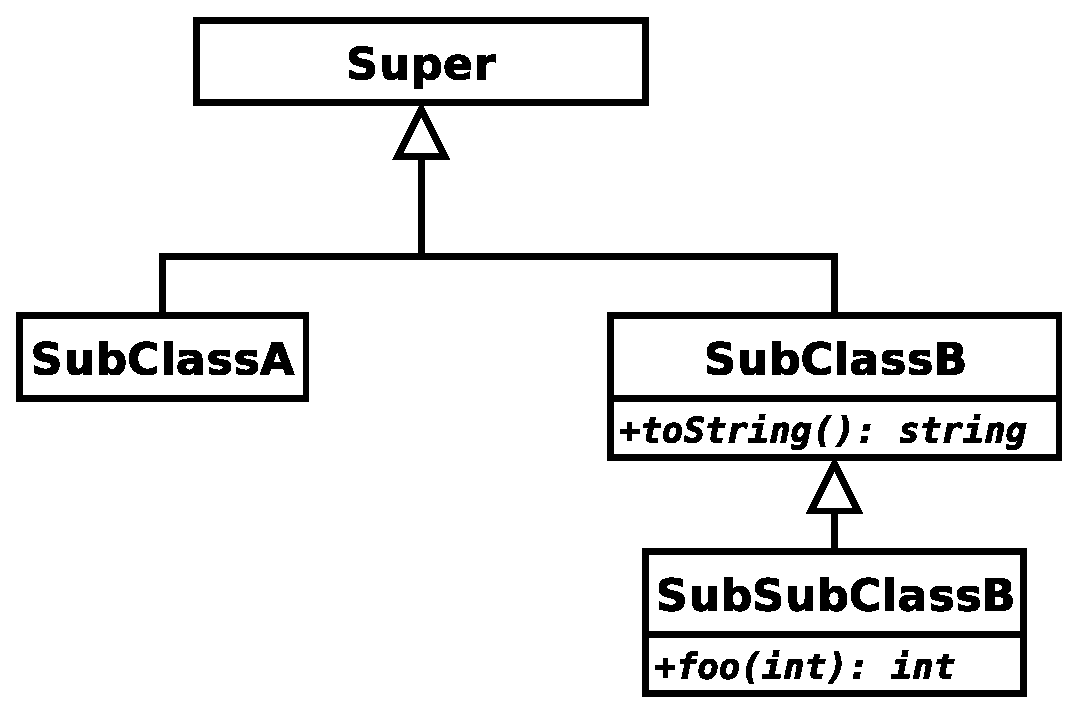
\includegraphics[width=\linewidth]{example-class-diagram.eps}
  \caption{Small example class hierarchy}
  \label{fig:class-hierarchy}
\end{figure}

Figure~\ref{fig:class-hierarchy} shows a small class hierarchy with
four classes.  Where \classname{SubClassA} and \classname{SubClassB}
are subclasses of the class \classname{Super} and
\classname{SubSubClassB} is a subclass of \classname{SubClassB}.  We
shall go through the different parts of the encoding of a class.

\begin{description}
\item[Class type]
\item[Subtyping/Inheritance]  
\item[Method]
\item[Constructor]  
\end{description}
 
\begin{ednote}{Ken}
  * Phantom types are inheritance paths.

  * We have one witness type per subtype.
  
  * We get upcasts for free.
  
  * Use base for plumbing.

  * Only single-inheritance is handled.
\end{ednote}


Continuing our running example the two widgets
\textit{window} and \textit{button} gets the following
types
\begin{displaymath}
\tApp{(\tApp{(\tApp{\tApp{(\tApp{\tBase}{\tWitness{window}})}
                   {\tWitness{container}}})}
            {\tWitness{widget}})}
     {\tName{t}}
\end{displaymath}
and
\begin{displaymath}
\tApp{(\tApp{(\tApp{(\tApp{\tBase}{\tWitness{button}})}
                 {\tWitness{container}})}
           {\tWitness{widget}})}
     {\tName{t}}
\end{displaymath}
(parenthesized here for readability). This tells us, reading from left
to right, that \textit{window} is a Window widget that extends the
Container widget, which in turn extends the Widget widget; similarly
for \textit{button}. It also tells us that \textit{window} and
\textit{button} have a common ancestor, namely the Container widget.
In particular, therefore, we can use both the window and the button in
all contexts expecting a Container.

For example, the function \texttt{Container.add} has type
\begin{displaymath}\begin{array}{l}
(\tApp{\tApp{\tApp{\alpha}{\tWitness{container}}}{\tWitness{widget}}}{\tName{t}})
\rightarrow
(\tApp{\tApp{\beta}{\tWitness{widget}}}{\tName{t}})
\\
\multicolumn{1}{r}{\rightarrow{\tUnit}}
\end{array}\end{displaymath}
from which we conclude that \texttt{Container.add} expects two arguments:
one which has to be a sub-widget of Container, and one which has to be
a sub-widget of Widget; the function returns the unit value. Considering
the types of \textit{window} and \textit{button} above, we see that
the application
\begin{displaymath}
\texttt{Container.add}\,\textit{window}\,\textit{button}
\end{displaymath}
is well-typed because \textit{window} is indeed a sub-widget of 
Container, and \textit{button} is indeed a sub-widget of Widget.

Consider now another function that only works on Buttons, \texttt{Button.set\_label}, with type
\begin{displaymath}\begin{array}{l}
(\tApp{\tApp{\tApp{\tApp{\alpha}{\tWitness{button}}}{\tWitness{container}}}{\tWitness{widget}}}{\tName{t}})
\rightarrow
\tString
\\
\multicolumn{1}{r}{\rightarrow\tUnit}
\end{array}\end{displaymath}
Thus \texttt{Button.set\_label} expects a sub-widget of Button and a string and returns unit.
If we were to apply this function to \textit{window} as in
\begin{displaymath}
\texttt{Button.set\_label}\,\textit{window}
\end{displaymath}
we would get a (compile-time) type error saying (essentially) that
a Window widget cannot be considered a Button widget because the
inheritance paths do not match. Here is the concrete message output
by the Moscow ML compiler
\begin{verbatim}
- Button.set_label window "New label";
! Toplevel input:
! Button.set_label window "New label";
!                  ^^^^^^
! Type clash: expression of type
!   base window_t container_t widget_t t
! cannot have type
!   'a button_t container_t widget_t t
\end{verbatim}

\begin{ednote}{Henning}
  Explain the cool signal thing.
\end{ednote}

\section{Process}
\label{sec:process}

\begin{ednote}{Henning}
  Fra mini muck-up til fuld toolkit
\end{ednote}

\begin{ednote}{Henning}
  What is a binding?
\end{ednote}

In constructing the \mgtk binding we leverage the foresightedness of
the \gtk developers. Early on it was recognized that it would be
important to have a machine-readable ``specification'' of the toolkit.
Essentially the specification would specify the widget classes, the
inheritance hierarchy, and methods and functions in the toolkit. The
specification became known as the \texttt{gtk.defs} file. One could
argue that it is simple enough to extract the same information from
the C header files; however, that incurs an initial hurdle in the
form of a suitable parser that is not present with the easily parsable
defs-format.

\begin{ednote}{Henning} This is crap, but it is there. \end{ednote}

The bulk of the \mgtk binding is constructed automatically from the
\texttt{gtk.defs} file. Based on this automatic construction the
complete binding process is naturally divided in two phases: (1)
binding ``design'', and (2) binding construction. It is important to
note here that the design phase can be carried out for a very small
subset of the complete toolkit after which the construction phase
``mimics'' that for the complete toolkit We refer to the design as a
\emph{muck-up} and the result as \minimgtk. This phase separation
makes it easier to get the design right simply because there are fewer
issues to deal with, and it makes the work involved in moving the
binding to other \sml compilers manageable (essentially just ask the
compiler writers to provide the equivalent of \minimgtk for their
compiler; and mimic that during the construction phase). Of course it
also when new releases of \gtk are produced. Most of the work in
constructing the binding for the new release is over when the muck-up
has been completed.

Let us return to our running example, and look at some example
specifications of widgets, functions, and signals. Figure~\ref{fig:gtk-defs}
shows three entries in the \texttt{gtk.defs} file.
\begin{figure}[htbp]
\begin{centering}
\begin{verbatim}
(define-object Button
  (in-module "Gtk")
  (parent "GtkBin")
  (c-name "GtkButton")
  (gtype-id "GTK_TYPE_BUTTON")
)

(define-function 
       gtk_button_new_with_label
  (c-name 
       "gtk_button_new_with_label")
  (return-type "GtkWidget*")
  (parameters
    '("const-gchar*" "label")
  )
)

(define-signal clicked
  (of-object "GtkButton")
  (return-type "void")
  (when "first")
)
\end{verbatim}
\caption{\texttt{gtk.defs} excerpt.\label{fig:gtk-defs}}
\end{centering}
\end{figure}
The first entry shows the shape of widget specification (defining
\texttt{Button} to be a sub-widget of \texttt{Bin}). The next entry
shows a function specification (that actually is constructor for the
\texttt{Button} widget) with return type \texttt{GtkWidget*} (in the C
implementation) and a string argument. Finally, we show a specification
of a signal on buttons.

\subsection{Stubs and code generation}
\label{sec:stubs-code-gener}





\section{Synergy}
\label{sec:synergy}

\begin{ednote}{Henning}
  SML + Gtk+ er godt
\end{ednote}



\section{Supported \sml compilers}
\label{sec:supp-sml-comp}

\begin{ednote}{Henning}
  MLton og Moscow ML (SML.NET med Gtk\#?)
\end{ednote}


\section{Related work}
\label{sec:related-work}

 Brainstorm of related work:
\begin{itemize}
\item SML-GTK 
\url{http://www.cs.nyu.edu/phd_students/leunga/sml-gtk/sml-gtk.html}

\item gtk+hs
\url{http://www.cse.unsw.edu.au/~chak/haskell/gtk}

\item lablgtk
\url{http://wwwfun.kurims.kyoto-u.ac.jp/soft/olabl/lablgtk.html}

\item sml\_tk
\url{http://www.informatik.uni-bremen.de/~cxl/sml_tk}

\item erlgtk
\url{http://erlgtk.sourceforge.net}


\item SWIG also used to generate language bindings

\item ``Calling Heaven from Hell''

\item nlffi

\end{itemize}



\section{Future Work}
\label{sec:future-work}

\begin{itemize}
\item Wrap all the libraries in the GNOME development platform
\end{itemize}



\section{Conclusion}
\label{sec:conclusion}

In this paper we have demonstrated that is theoretical and practically
possible to make an interface from SML to GTK.

\bibliographystyle{alpha}
\bibliography{mgtk}

\end{document}

%%% Local Variables: 
%%% mode: latex
%%% TeX-master: t
%%% End: 

% LocalWords:  mGTK FREENIX Friis Niss GtkBasis fn wildcard tl gtk defs SML
% LocalWords:  GtkWidget MLton mgtk
